\sectionquestion{S22 TA Questions Go Here!}

\begin{parts}


\part Neural the Narwhal has recently started texting with his other narwhal friends, but, as it turns out, narwhals aren't great at spelling. He realizes that his friends tend to only make substitution mistakes, i.e., replacing a letter for another, and \textbf{not} addition (having extra letters) or deletion (missing letters) mistakes. Having taken an ML course at CMU, Mr. Narwhal decides to build a spelling correction model for his friends using a hidden Markov model (HMM).
\begin{subparts}
\subpart[1] During training, what data should he use for the observations $\xv^{(i)}$?
\begin{tcolorbox}[fit,height=2cm, width=15cm, blank, borderline={1pt}{-2pt}]
%solution
\begin{soln}
Raw text message data from Narwahl's friends, which contain incorrect spellings.
\end{soln}
\end{tcolorbox}

\subpart[1] During training, what data should he use for the hidden states $\yv^{(i)}$?
\begin{tcolorbox}[fit,height=2cm, width=15cm, blank, borderline={1pt}{-2pt}]
%solution
\begin{soln}
A copy of $\xv^{(i)}$ with the misspellings corrected.
\end{soln}
\end{tcolorbox}

 \uplevel{ Mr. Narwhal was able to train an HMM. During testing, however, he notices that uncommon misspellings have zero probability according to his model. }
\subpart[1] What is the likely reason for this problem?
\begin{tcolorbox}[fit,height=2cm, width=15cm, blank, borderline={1pt}{-2pt}]
%solution
\begin{soln}
An uncommon misspelling (e.g. t as z) could have a zero emission probability, or zero transition probability in the parameters because it is never seen in the training set. 
\end{soln}
\end{tcolorbox}


\subpart[1] Describe a way to address this problem?
\begin{tcolorbox}[fit,height=2cm, width=15cm, blank, borderline={1pt}{-2pt}]
%solution
\begin{soln}
MAP estimation, Laplacian smoothing / Add-1 / Add-K
\end{soln}
\end{tcolorbox}

% REMOVED
% \subpart[1] Give a possible way that this solution may act in an undesirable way.
% \begin{tcolorbox}[fit,height=2cm, width=15cm, blank, borderline={1pt}{-2pt}]
% %solution
% \begin{soln}
% Weighing all unobserved events the same may lead to incorrect predictions.
% \end{soln}
% \end{tcolorbox}

\end{subparts}
\begin{qauthor}
Abu, (1) Talk about ‘Autocorrect’ as an HMM problem; (2) Smoothing - Laplacian advantages / disadvantages.

(Zack feedback): Really cool HMM question! If there's a way to make the preamble a little shorter and give a little more of a hint to (a) and (b), as I'm not sure if autocorrect through HMMs is immediately intuitive. Also for the refsol, I think (b) should also allow "Words \textit{intended} to be written".

Abhi: Not sure that this actually matches a learning objective - most of them seem to be about the model itself rather than applying the model to tasks or discussing smoothing. As Zack said, it may be unintuitive (especially to people who have not taken NLP or are not familiar with the noisy channel model), and students might not be preparing for this when there is so much content directly on the learning objectives.

In terms of preamble wording, I think that introducing addition and deletion as possible mistakes might be more confusing. We might want to just say "only substitution mistakes" + define substitution and leave it as that.

Parts (a) and (b) seem like they could be very open to "interesting" student answers that they might be regrade trigger-happy about.

The discussion between parts (b) and (c) could maybe be made more targeted to guide people towards the answer for part (c). An example could be "he was able to train an HMM on a large number of common spelling mistakes and true spellings."

Part (c) seems fine in terms of specificity, but part (d) should be graded with respect to part (c) for consistency points in the case that someone puts down a different answer for part (c).

Tara: Agreed on the setup being unintuitive especially given that when we taught HMM's, we motivated it by thinking of hidden states as expected/predicted categorization of the output. Not sure students will see how this maps to the correct next letter being predicted vs observed. 

\end{qauthor}


\part Neural and his friend Cilantro are observing the Instagram$^{\text{TM}}$ posts of their fellow course mascots. They decide all posts can be labeled in one of two categories: Announcements or Jokes which we will denote as A and J, respectively. For simplicity, all observed posts are described using a one word descriptor. They also notice that the feeds follow a first order Markov assumption, and that each post is conditionally independent of all other posts given the category it belongs to. 
\begin{subparts}

\subpart[3]Suppose the mascots observe three posts from Neural's Instagram feed, Draw the graphical model which represents Neural's Instagram feed. Use $y_{1:3}$ to represent the category of the posts and $x_{1:3}$ to represent the posts.\\

\begin{tcolorbox}[fit,height=10cm, width=15cm, blank, borderline={1pt}{-2pt}]
    %solution
    
\end{tcolorbox}
\begin{soln}
\begin{center}
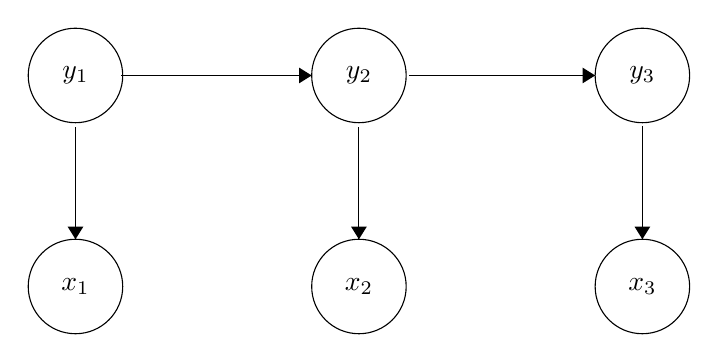
\begin{tikzpicture}[scale=0.2]
\tikzstyle{every node}+=[inner sep=0pt]
\draw [black] (3.3,-3.2) circle (3);
\draw (3.3,-3.2) node {$y_1$};
\draw [black] (21.3,-3.2) circle (3);
\draw (21.3,-3.2) node {$y_2$};
\draw [black] (39.3,-3.2) circle (3);
\draw (39.3,-3.2) node {$y_3$};
\draw [black] (3.3,-16.6) circle (3);
\draw (3.3,-16.6) node {$x_1$};
\draw [black] (21.3,-16.6) circle (3);
\draw (21.3,-16.6) node {$x_2$};
\draw [black] (39.3,-16.6) circle (3);
\draw (39.3,-16.6) node {$x_3$};
\draw [black] (6.2,-3.2) -- (18.3,-3.2);
\fill [black] (18.3,-3.2) -- (17.5,-2.7) -- (17.5,-3.7);
\draw [black] (24.5,-3.2) -- (36.3,-3.2);
\fill [black] (36.3,-3.2) -- (35.5,-2.7) -- (35.5,-3.7);
\draw [black] (3.3,-6.5) -- (3.3,-13.6);
\fill [black] (3.3,-13.6) -- (3.8,-12.8) -- (2.8,-12.8);
\draw [black] (21.3,-6.5) -- (21.3,-13.6);
\fill [black] (21.3,-13.6) -- (21.8,-12.8) -- (20.8,-12.8);
\draw [black] (39.3,-6.4) -- (39.3,-13.6);
\fill [black] (39.3,-13.6) -- (39.8,-12.8) -- (38.8,-12.8);
\end{tikzpicture}
\end{center}
\end{soln}
\subpart[3]
Write down the factorization of the above model.
\begin{tcolorbox}[fit,height=3cm, width=15cm, blank, borderline={1pt}{-2pt}]
    %solution
    \begin{soln}
    $P(y_1)P(y_2|y_1)P(y_3|y_2)P(x_1|y_1)P(x_2|y_2)P(x_3|y_3)$
    \end{soln}
\end{tcolorbox}

\subpart[2] In an observed Instagram feed of length $T$ which of the following are true? Assume that $t\in \{1,\dots,T\}$
\begin{checkboxes}
     \choice $x_t \perp \!\!\! \perp x_{t-1}\ |\ y_t$
     \choice $x_{t-2}\perp \!\!\! \perp y_t\ |\ y_{t+1}$
     \choice $y_t \perp \!\!\! \perp y_{1:t-2}\ |\ y_{t-1}$
     \choice $x_t \perp \!\!\! \perp x_{t-1}\ |\ y_{t+1}$
     \choice $y_t \perp \!\!\! \perp y_{t-2}\ |\ x_{t+1}$
    \end{checkboxes}
    \begin{soln}
    A,C
    \end{soln}
    
    \subpart[2] Help Cilantro and Neural by performing the training step of their model by calculating the Initial, Transition, and Emission matrices on the following data.\\
    
    \textbf{Training set:} 
    \begin{verbatim}
    reel     J
    photo     A
    story    J
    
    reel     J
    story    A
    photo     J
    
    story     A
    photo    J
    \end{verbatim}
    
    
    Initial:
    \begin{tcolorbox}[fit,height=3cm, width=5cm, blank, borderline={1pt}{-2pt}]
    %solution
    \begin{soln}
    
    \end{soln}
    \end{tcolorbox}
    
    
    Transmission:
    \begin{tcolorbox}[fit,height=3cm, width=5cm, blank, borderline={1pt}{-2pt}]
    %solution
    \begin{soln}
    
    \end{soln}
    \end{tcolorbox}
    
    
    Emission:
    \begin{tcolorbox}[fit,height=3cm, width=5cm, blank, borderline={1pt}{-2pt}]
    %solution
    \begin{soln}
    
    \end{soln}
    \end{tcolorbox}


\end{subparts}
    \begin{qauthor}
    (1) Tara Lakdawala, (2) HMM \& Bayes Nets
    
    (Zack feedback): Honestly, I thought this could be harder lmao, besides part (c) I think is well callibrated.
    \end{qauthor}
    
    


\part Consider the following generative story, where each event is tagged with the corresponding variable name:
\begin{enumerate}
    \item Matt has been studying the nature of the multiverse for years, and finally has developed a machine to project his mind into a different universe ($X_1$).
    \item Despite the protests of Joshmin and Brynn, who fear for the safety of the multiverse, Matt turns on his machine ($X_2$).
    \item At the same time all this is happening, Evil-Matt from Earth-10601 has also developed a multiverse machine ($X_3$).
    \item Evil-Matt then turns on his machine ($X_4$).
    \item Because of both machines turning on, reality collapses ($X_5$).
    \item Nueral, the great overlord of the multiverse, now has to restart their universes to account for Matt and Evil-Matt's meddling ($X_6$).
\end{enumerate} 
Note that this implies the following conditional independence assumptions:
\begin{itemize}
    \item $(X_1, X_2) \perp (X_3, X_4)$
    \item $X_1 \perp X_5 \mid X_2$
    \item $X_3 \perp X_5 \mid X_4$
    \item $(X_1, X_2, X_3, X_4) \perp X_6 \mid X_5$
    \item $(X_1, X_2) \not\perp (X_3 ,X_4) \mid X_5 \cup X_6$
\end{itemize}

\begin{qauthor}
    Abhi: have they seen this notation with parentheses or the union before (and is the union actually supposed to be a union)? they might get confused as to what it means
    (also is Nueral intentional as some sort of evil Neural)
\end{qauthor}

Additionally, you may assume that all the edges only can go from lower-number variables to higher (e.g. $X_1 \rightarrow X_2$), as time flows only in one direction.

\begin{qauthor}
    Abhi: is it worth it to stick this assumption only on the parts that use it instead of on the general description of the problem setting
\end{qauthor}

\begin{subparts}
\subpart[3] Given the generative story and the set of explicit conditional independence relations, draw the Bayesian network that represents this story.
\begin{tcolorbox}[fit,height=10cm, width=15cm, blank, borderline={1pt}{-2pt}]
    %solution
    
\end{tcolorbox}
\begin{soln}
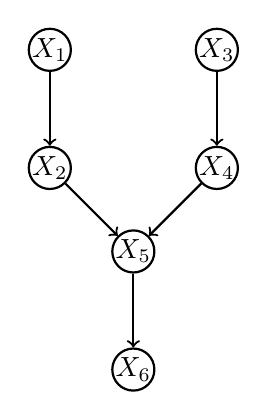
\begin{tikzpicture}[node distance={15mm}, thick, main/.style = {draw, circle}] 
\node[main] (1) {$X_1$}; 
\node[main] (2) [below of=1] {$X_2$}; 
\node[main] (5) [below right of=2] {$X_5$}; 
\node[main] (4) [above right of=5] {$X_4$}; 
\node[main] (3) [above of=4] {$X_3$}; 
\node[main] (6) [below of=5] {$X_6$};
\draw[->] (1) to (2);
\draw[->] (2) to (5);
\draw[->] (3) to (4);
\draw[->] (4) to (5);
\draw[->] (5) to (6);
\end{tikzpicture} 
\end{soln}
\begin{qauthor}
    (1)Zack, (2) Bayes Nets from independence assumptions
\end{qauthor}



\subpart[3] Just as Joshmin and Brynn had feared, because of Matt and Evil-Matt's tampering with the Multiverse, the very fabric of time itself broke down as well! Thus, \textbf{we now drop the assumption that all edges must go from lower to higher}. Now draw a \textit{\textbf{different}} Bayes net from your answer in part (a) that satisfies the \textit{\textbf{same}} conditional independence assumptions. \textit{(Hint: you may have to include an edge that goes from higher to lower, e.g. $X_6 \rightarrow X_5$)}
\begin{tcolorbox}[fit,height=10cm, width=15cm, blank, borderline={1pt}{-2pt}]
    %solution
    
\end{tcolorbox}
\begin{soln}
Namely, the only change we can make is to flip the initial edges from $X_1$ to $X_2$ and/or $X_3$ to $X_4$, as we can't reorient any other edges as that would change the collider structure.
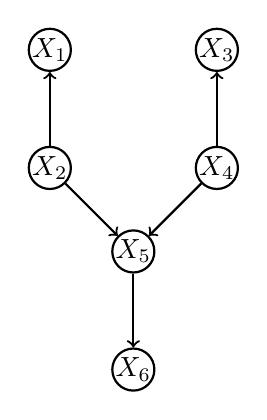
\begin{tikzpicture}[node distance={15mm}, thick, main/.style = {draw, circle}] 
\node[main] (1) {$X_1$}; 
\node[main] (2) [below of=1] {$X_2$}; 
\node[main] (5) [below right of=2] {$X_5$}; 
\node[main] (4) [above right of=5] {$X_4$}; 
\node[main] (3) [above of=4] {$X_3$}; 
\node[main] (6) [below of=5] {$X_6$};
\draw[->] (2) to (1);
\draw[->] (2) to (5);
\draw[->] (4) to (3);
\draw[->] (4) to (5);
\draw[->] (5) to (6);
\end{tikzpicture} 
\end{soln}
\begin{qauthor}
    (1)Zack, (2) Bayes Nets from independence assumptions
    
    Abhi: grading might be really rough here if they mess up part a (e.g. could put the answer for a down for b. Could we perhaps make explicit that time has to flow backward somewhere in the answer for b?
    
    Zack: Added a hint so that they at least know they should have some backwards edge
\end{qauthor}

\subpart[2] More generally, consider the situation where we only have three nodes in our Bayesian network $X$, $Y$, and $Z$. What can we say about the relationship between common-parent structures (e.g. $X \leftarrow Y \rightarrow Z$), cascade structures ($X \rightarrow Y \rightarrow Z$), and v-structures ($X \rightarrow Y \leftarrow Z$) in terms of the conditional independence assumptions they imply when conditioning / not conditioning on $Y$?
    \begin{checkboxes}
     \choice Common-parent structures and cascade structures imply the same independence assumptions, but these are different than what is implied by v-structures.
     \choice Common-parent structures and v-structures imply the same independence assumptions, but these are different than what is implied by cascade structures.
     \choice Cascade structures and v-structures imply the same independence assumptions, but these are different than what is implied by common-parent structures.
     \choice Common-parent, cascade, and v- structures all imply different sets of conditional independencies.
     \choice Common-parent, cascade, and v- structures all imply the same set of conditional independencies.
    \end{checkboxes}
\begin{soln}
    A.
\end{soln}
\begin{qauthor}
    (1)Zack, (2) Bayes Nets and independence assumptions
    
    Abhi: we should make sure the terminology for each  structure matches the terminology we give in class. Can we also somehow make this more explicitly targeted to the cases Y is conditioned on and Y is not conditioned on so they have a direction to go off of?
    
    Zack: changed "collider" to v-structure, and reformatted question to talk specifically about conditioning on $Y$.
\end{qauthor}
\end{subparts}



\part[1] Let $f(x) = 0.5x^2 + x^4$. Report the value of $x$ after a single update using fixed point iteration. Initialize $x=2$. 

\begin{tcolorbox}[fit,height=1cm, width=2cm, blank, borderline={1pt}{-2pt}]
%solution
\begin{soln}
-32
\end{soln}
\end{tcolorbox}

\begin{soln}
An explanation: 
$$\frac{\partial}{\partial x}f(x) = 0 = x + 4x^3$$
$$x^{(t+1)} = -4x^3$$
$$x^{(t+1)} = -32$$
\end{soln}

\begin{qauthor}
(1) Sana, (2) RL 1d. Explain how to solve a system of equations using fixed point iteration, (3) 1 point for correct answer

Sana: We spent about 10 mins on fixed point iteration in lecture and there are a good number of slides about it, but I can't help but wonder if this is fair given so many of the other major topics we cover in this module? If this section is too long maybe we should drop this. Thoughts?

Abhi: tangential, but i believe this converges to 0 only for starting values $< 0.5$, oscillates $0.5$ to $-0.5$, and explodes for higher values. This might be a bit weird for students if they were taught to think of fixed points as attractors without nuance in selection of starting value. 
\end{qauthor}


\part In this question, you will compare the computational complexities of value iteration and policy iteration.

\begin{subparts}
\subpart[1] \textbf{Numerical answer:} What is the computational complexity of choosing the best action \textbf{for a single state}, given the value function and reward function?
\begin{tcolorbox}[fit,height=1cm, width=2cm, blank, borderline={1pt}{-2pt}]
%solution
\end{tcolorbox}
\begin{soln}
$O(|A| |S|)$ (argmax over actions and sum over states)
\end{soln}
\begin{qauthor}
Abhishek Vijayakumar, Reinforcement Learning 1.f Contrast the computational complexity and empirical convergence of value iteration vs. policy iteration
\end{qauthor}

\subpart[1] \textbf{Numerical answer:} What is the computational complexity of solving the system of Bellman equations for a fixed policy to compute the value function values for all states for that policy?
\begin{tcolorbox}[fit,height=1cm, width=2cm, blank, borderline={1pt}{-2pt}]
%solution
\end{tcolorbox}
\begin{soln}
$O(|S|^3)$ (system of $S$ equations)
\end{soln}
\begin{qauthor}
Abhishek Vijayakumar, Reinforcement Learning 1.f Contrast the computational complexity and empirical convergence of value iteration vs. policy iteration
\end{qauthor}

\subpart[1] \textbf{Numerical answer:} What is the computational complexity of one iteration of value iteration?
\begin{tcolorbox}[fit,height=1cm, width=2cm, blank, borderline={1pt}{-2pt}]
%solution
\end{tcolorbox}
\begin{soln}
$O(|A| |S|^2)$
\end{soln}
\begin{qauthor}
Abhishek Vijayakumar, Reinforcement Learning 1.f Contrast the computational complexity and empirical convergence of value iteration vs. policy iteration
\end{qauthor}

\subpart[1] \textbf{Numerical answer:} What is the computational complexity of one iteration of policy iteration?
\begin{tcolorbox}[fit,height=1cm, width=2cm, blank, borderline={1pt}{-2pt}]
%solution
\end{tcolorbox}
\begin{soln}
$O(|A| |S|^2 + |S|^3)$
\end{soln}
\begin{qauthor}
Abhishek Vijayakumar, Reinforcement Learning 1.f Contrast the computational complexity and empirical convergence of value iteration vs. policy iteration
\end{qauthor}

\subpart[1] \textbf{Select one:} Which algorithm usually converges in fewer iterations?
\begin{checkboxes}
 \choice Value Iteration
 \choice Policy Iteration
\end{checkboxes}
\begin{soln}
B
\end{soln}
\begin{qauthor}
Abhishek Vijayakumar, Reinforcement Learning 1.f Contrast the computational complexity and empirical convergence of value iteration vs. policy iteration

Sana: Do we want to add something about this being empirically rather than theoretically just in case or is that already understood? I might be nitpicking

Abhi: i think usually implies in practice/empirically, but i'd be down to change it to being explicitly empirically unless someone can cite a theoretical result
\end{qauthor}
    
\end{subparts}


\part Answer the following questions about the Bellman equation.
\begin{subparts}
\subpart[1] Write the general form of the Bellman equation corresponding to a policy $\pi$, reward function $R(s,a)$ where $s$ is a state and $a$ is an action, and state space $S$.
\begin{tcolorbox}[fit,height=2cm, width=15cm, blank, borderline={1pt}{-2pt}]
%solution
\begin{soln}
$V^{\pi}(s) = R(s, \pi(s))  + \gamma \sum_{s' \in S} p(s' | s, \pi(s))V^{\pi}(s') $
\end{soln}
\end{tcolorbox}

\subpart[1] Explain what the equations above encapsulate in simple terms.
\begin{tcolorbox}[fit,height=2cm, width=15cm, blank, borderline={1pt}{-2pt}]
%solution
\begin{soln}
The value function at a certain state can be decomposed into two subparts: the immediate reward, and a future discounted reward that can be expressed as a recursive relationship
\end{soln}
\end{tcolorbox}
\end{subparts}
\begin{qauthor}
        Abu, Bellman equations
        
Sana: This first question feels a lot like a ``did you write the formula on the cheat sheet" question to me, maybe we can reformulate this to not have as much of that? The second one is better, but again ``expected total future discounted reward" is something we have said enough times that this question may not be testing anything substantial. We could, however, ask them to ``dissect" that formula. ie: match the parts of the formula that correspond to, ``expected", ``total", ``future", ``discounted", and ``reward." Though still quite easy, this will be a better test than the question outlined here. Lastly, ``simple terms" is still inviting a possible essay. If we are to keep this question, we should change the language to control for that.

Abhi: Specifically, we might also want $R(s, a, s')$ instead of $R(s, a)$. Part b also feels like it is too vague to actually grade while discriminating surface understanding from deep understanding of the intuition behind each part of the equation.
\end{qauthor}


\part Suppose we are doing deep Q-learning with true loss function
$$\ell (\Wv) = \sum_{s \in \mathcal{S}} \sum_{a \in \mathcal{A}} f\left( Q^* (s, a) - Q(s, a; \Wv) \right)$$
where
$$f(z) = e^z + e^{-z}$$
which we wish to optimize using temporal difference learning.

\begin{subparts}
\subpart[2] What component of this loss function do we approximate with the temporal difference target?
\begin{tcolorbox}[fit,height=1.5cm, width=2.5cm, blank, borderline={1pt}{-2pt}]
%solution
\end{tcolorbox}
\begin{soln}
$Q^* (s, a)$
\end{soln}
\begin{qauthor}
RL 2b Implement Q-learning
\end{qauthor}

\subpart[2] Write an expression for the temporal difference target. Assume $r = R(s, a, s')$ and that the discount factor is $\gamma$. Write your answer in terms of $r, s, a, s', \text{ and } \Wv.$
\begin{tcolorbox}[fit,height=1.5cm, width=15cm, blank, borderline={1pt}{-2pt}]
%solution
\end{tcolorbox}
\begin{soln}
$r + \gamma \max_{a'} Q(s', a'; \Wv)$
\end{soln}
\begin{qauthor}
RL 2b Implement Q-learning

Abhi - should we add "in terms of?"
Sana: I added one in for now, @matt leaving the final word to you
\end{qauthor}

\subpart[1] \textbf{Select one:} Why is this objective computationally infeasible to compute, even with our using our temporal difference target to approximate the component from part (a)?
\begin{checkboxes}
 \choice The action space $\mathcal{A}$ is unknown.
 \choice The state space $\mathcal{S}$ is too large.
 \choice The parameters $\Wv$ are not fully specified.
 \choice $f$ is exponential in its input, and only linear functions are computationally feasible when performing deep Q-learning.
\end{checkboxes}
\begin{soln}
B. A is wrong because actions are known, C is wrong because the parameters are fully specified, and D is wrong because the exponential here means nothing about computational feasibility.
\end{soln}
\begin{qauthor}
RL 2b Implement Q-learning
\end{qauthor}

\subpart[1] \textbf{Select one:} What should we do to have a computationally feasible optimization process?
\begin{checkboxes}
\choice Apply a two-hot encoding to the action space to encapsulate all possible actions, then use this encoding instead of directly summing over actions.
\choice Perform SGD, instead approximating and optimizing $\left( Q^* (s, a) - Q(s, a; \Wv) \right)^2$ for a single $(s, a)$ pair each iteration.
\choice Approximate the parameter matrix $\Wv$ with a parameter vector $\wv$ and bias term $b$.
\choice Replace our exponential function $f(z) = e^z + e^{-z}$ with the piecewise linear absolute value function $f(z) = |z|$.
\end{checkboxes}
\begin{soln}
B. Each answer corresponds to an answer of the above part, and the answers for A, C, and D are made nonsensical on purpose.
\end{soln}
\begin{qauthor}
RL 2b Implement Q-learning
\end{qauthor}

\end{subparts}


\part[1] \textbf{Select all that apply.} In which of the following situations would we be very likely to benefit from dimensionality reduction?
    {%
    \checkboxchar{$\Box$} \checkedchar{$\blacksquare$} % change checkbox style locally
    \begin{checkboxes}
     \choice We are training a logistic regression model on high-dimensional bag-of-words vectors and we need to create more explainable features.
     \choice We are attempting to perform K-Means on high-dimensional vectors, but the computation is taking too long to run each iteration.
     \choice We are training a multiclass classification model on high-dimensional inputs, but it keeps overfitting to noise in the data.
     \choice None of the above
    \end{checkboxes}
    }
    \begin{soln}
    B, C. For B, lower dimensional data will reduce the runtime. For C, generally the dimensions we remove correspond to noise. A would not be selected because bag of words features are very explainable, but the dimensionality reduction might create uninterpretable combinations of features/words.
    \end{soln}
    \begin{qauthor}
    Abhi, Learning Paradigms 4.b Identify examples of high dimensional data and common use cases for dimensionality reduction
    
    (Zack Feedback): I feel like there could be a better negative option for C, as I feel like a lot of students will focus on the first half and not the 'explainable' part and even then, they might try to argue that 'the directions that maximize the variance' are more explainable or something. Though probably fine to leave as is.
    
    Tara: this one is subtle (ie. requires good reading comprehension) which is not super compatible with exam brains. I'd try to see if we can make it slightly easier to catch onto the "explainable features" part of option C
    
    Abhi: agree with the above comments, will attempt rewordings for option C (open to suggestions)
    
    Sana: how about some variant of ``We are building an interpretable logistic regression classifier on bag-of-words vectors and want to add more explainable features"? This isn't much of a change but it does emphasize interpretability/explainability, something we lose with PCA.
    \end{qauthor}
    

\part[1] For a zero-mean dataset, the reconstruction error can be expressed as: $$\argmin_{\mathbf{v}: \|\mathbf{v}\|^2 = 1} \frac{1}{N} \sum_{i=1}^{N} \| x^{(i)} - (v^{T}x^{(i)})v\|^{2}$$ Show that this is equivalent to maximizing variance of the projected vector.\\

    \begin{tcolorbox}[fit,height=7cm, width=15cm, blank, borderline={1pt}{-2pt}]
                %solution
            
        \begin{soln}
            $$\argmin_{\mathbf{v}: \|\mathbf{v}\|^2 = 1} 
            \frac{1}{N} \sum_{i=1}^{N} \| x^{(i)} - (v^{T}x^{(i)})v\|^{2}$$
            
            $$\argmin_{\mathbf{v}: \|\mathbf{v}\|^2 = 1}
            \frac{1}{N} \sum_{i=1}^{N} \| x^{(i)} \|^{2} - (v^{T}x^{(i)})^2$$
            
            $$\argmax_{\mathbf{v}: \|\mathbf{v}\|^2 = 1} \frac{1}{N} \sum_{i=1}^{N} (v^{T}x^{(i)})^2$$
        \end{soln}
    \end{tcolorbox}
        \begin{qauthor}
        Udai
        
        Tara: added a solution box here. Also need to specify the level to which students should simplify answers (ie. nobody should leave intermediate steps as an answer and get full credit)
        
        Abhi: note that this isn't actually the reconstruction error, but an argmin producing the top principal component
        
        Sana: in light of the above comment maybe rephrase this as ``the vector that minimizes the reconstruction error can be expressed as...show that this is equivalent to the vector that maximizes the variance..."
        \end{qauthor}

    
\part[1] 
\textbf{Select One:} For a dataset of values $\{\begin{bmatrix}
           1 \\
           0 \\
           2
         \end{bmatrix}, \begin{bmatrix}
           2 \\
           5 \\
           6
         \end{bmatrix}, \begin{bmatrix}
           4 \\
           12 \\
           4
         \end{bmatrix}\}$, what is the covariance between index 0 and 2?
\begin{quote}

\begin{list}{}
     \item\Circle{} 2/3
     \item\Circle{} 5/3
     \item\Circle{} 1/3
     \item\Circle{} None of the Above
\end{list}
\end{quote}

\begin{qauthor}
    A. 
    
    Udai. This tests students' understanding of covariance and ability to calculate covariance on a simple dataset.
    
    Abhi: this almost feels like we're testing prereq material that they both should know and probably don't know. We might also want to make life easier by mean-centering for them.
    
    Sana: big sad but seconding Abhi's comment that they might not know this
\end{qauthor}


\part[1] \textbf{True or False:} K-means minimizes intra-cluster variance.
    \begin{checkboxes}
     \choice True 
     \choice False
    \end{checkboxes}
    \begin{soln}
    True
    \end{soln}
    \begin{qauthor}
    Samiksha Kale, Learning Paradigms 3.b
    
    it might be a good idea to give them a mathematical definition of what we mean by intra-cluster variance (we might also want to specify the objective since we do that for a lot of K-means content)
    \end{qauthor}
    

%%%
\part

You are the chief engineer of Narwhal Music, a startup that is working on building a personalized music streaming application. Narwhal Music is new to the streaming industry and has to compete with streaming giants such as Spotify and Amazon Music. Besides, it only has access to the data that the users have provided during signup. This includes data such as the user’s age group and a list of preferred genres. Thankfully, you also have access to a large database containing information about all the songs recorded from the summer of 1969 to the present. A key offering of Narwhal Music is an AI Playlist, which consists of a playlist of recommended songs built on the fly for every user. Your task is to build this AI playlist with the resources at hand and improve this system continually so that you can deliver personalized music recommendations to each user. \\

For a new user, you decide to start by recommending a random song from your database belonging to a genre preferred by the user and collecting the user’s feedback (likes or dislikes) for the recommendation. If the user likes the recommended song, your strategy is to find the most similar song in the database and recommend it as the next recommendation. Assume that the similarity between songs is measured by computing the cosine distance between them and that each song in your database is expressed as an n-dimensional vector.


\begin{subparts}
\subpart[1] \textbf{Select one:} The approach stated above resembles which type of recommender system?
    \begin{checkboxes}
     \choice Content Based Filtering 
     \choice Collaborative Filtering
    \end{checkboxes}
    \begin{soln}
    Content Based Filtering
    \end{soln}
    \begin{qauthor}
    (1) Shubham Phal (2) Recommender system
    
    (Zack Feedback): Given the low weight of the question, it might be helpful to either A) reduce the question length a \textit{ton} in order to match the question weight or B) ask something more than just 2 2-choice 1-point questions.

    Abhi: edited somewhat for grammar, also echoing what Zack said about the length
    \end{qauthor}

\uplevel{
After running for over a month, Narwhal Music has made significant gains in its popularity. You now also have access to data such as user feedback for a song. You may notice that although the number of users signing up on Narwhal Music is growing, the user retention rate is still low. Upon investigating, you discover that the root cause of this problem is that users are getting bored of being continually recommended songs within the same genre. To fix this problem, you decide to improve the diversity of recommendations by recommending songs that are liked by other users who are in the same age group and have similar interests as the given user.
}

\subpart[1] \textbf{Select one:} The new approach described above resembles which type of recommender system?
    \begin{checkboxes}
     \choice Content Based Filtering 
     \choice Collaborative Filtering
    \end{checkboxes}
    \begin{soln}
    Collaborative Filtering
    \end{soln}
    \begin{qauthor}
    (1) Shubham Phal (2) Recommender system
    
    Abhi: edited somewhat for grammar, same issue as above with length. the bit about age group instead of just working with shard item preferences might be a bit confusing for people as well
    \end{qauthor}


\subpart[2] \textbf{Short answer:} State one problem with the new approach.
    \fillwithlines{8em}
    
    \begin{soln}
    No way to recommend a song that no user has interacted with
    \end{soln}
    \begin{qauthor}
    (1) Shubham (2) Recommender Systems
    
    Abhi: this seems very vague and might have many possible responses. it also is incorrect under one interpretation because new users seem to still be given random songs
    \end{qauthor}    
\end{subparts}
%%%
    
\end{parts}
